\chap{Conclusion}

\section{Summary}
During this study different Python utilities have been tested to show their potential in the Data Science field. 
\newpage
\section{Recommendations to future work}
\vspace{-5mm}
In this section are reported some ideas for future work and some extra implementation that have not been implemented during this thesis due to the time limitation. Some of them could be considered interesting for future reserach or analysis.
\begin{itemize}
\item \textbf{Improve the dataset content}\\ The data collection that has done during this thesis provides just public data about territorial statistics. Would be interesting to test the same system with data coming from single reality, like for example in this case gather data from a single locality of salmon farming and then run the system on it.
\item \textbf{Visualization of the data}\\ Also if the library used during this study allow a quite good visualization of the data, it would be useful to check out other ways to realize it, which could imply the use of Python or not. For instance, if you still want to use Python could be possible to check out other libraries, such as "Plotly Python Library".
\item \textbf{Improve the prediction system}\\ This is the part which has much more possible future works. Forecasting system development is today a fundamental issue that involves different area of studies. To achieve an accurate model and significant results it needs much more specific research than the one reported in this study, that was just for report a general idea about it. I strongly recommend to future work to research about Artificial intelligence methods, such as "Artificial Neural Networks".
\item \textbf{System as a service}\\ Would be really interesting to investigate about a possible way toprovide this kind of analysis, displaying and forecasting systems like a service.
\end{itemize}

%\begin{figure}[H]
%	\centering
%       \makebox[\textwidth][c]{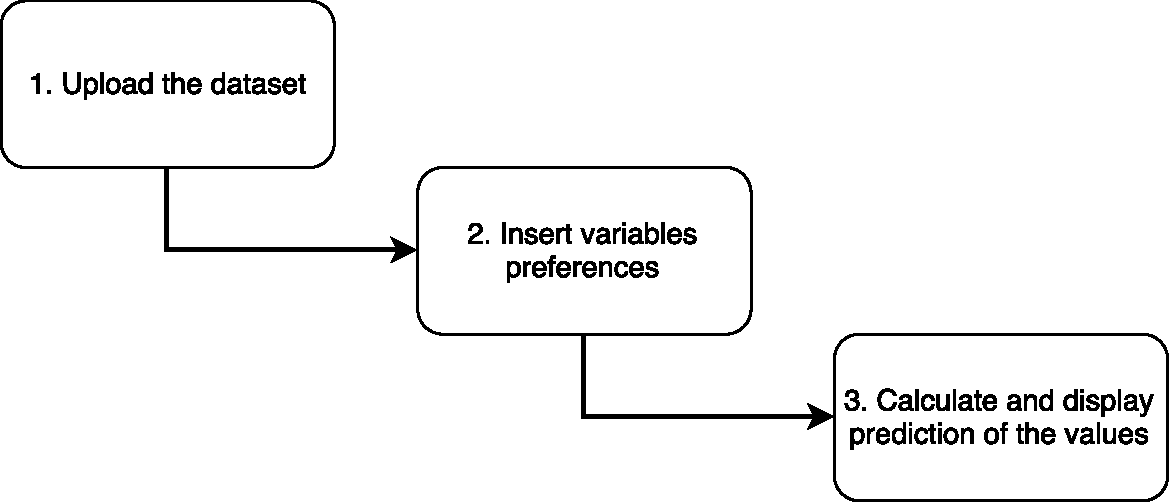
\includegraphics[width=1\textwidth]{Files/ServiceSystem.pdf}}
%    \caption{Idea of the Servie System for predictions.}
%\end{figure}







